\documentclass[a3paper,xelatex,english]{bxjsarticle}
\usepackage{pgfplots,pgfplotstable}
\pgfplotsset{ compat = newest }
\usepackage{tikz}
\usetikzlibrary{arrows.meta,bending,calc,shapes,positioning}
\usepackage{ascmac}
\usepackage{fancybox}
\usepackage{amsmath,amssymb}
\usepackage{algorithm}
\usepackage[edges]{forest}
\usepackage{array}
\usepackage{algpseudocode}
\usepackage{paralist}
\usepackage{cases}
\usepackage{fvextra}
\usepackage{colortbl}
\usepackage{xcolor}
\usepackage{fancyhdr}
\usepackage[explicit]{titlesec}
\usepackage{xspace}
\usepackage[many]{tcolorbox}
\usepackage{lastpage}
\usepackage{verbatim}
\usepackage{multirow}
\usepackage{censor}
\usepackage[unicode,pdftitle={Report of Entropy estimates based on NIST SP 800-90B non-IID track},setpagesize=false]{hyperref}
\usepackage[open,openlevel=4]{bookmark}
\newcommand\mib[1]{\boldsymbol{#1}}
\usepgfplotslibrary{patchplots}
%%%%%%%%%%%%%%%%%%%%%%%%%%%%%%%%%%%%%%%%%%%%%%%%%%%%%%%%%%%%%%%%%%%%%%%%%%%%%%%
%%%%%%
%%%%%% customize page numbering
%%%%%%
%%%%%%%%%%%%%%%%%%%%%%%%%%%%%%%%%%%%%%%%%%%%%%%%%%%%%%%%%%%%%%%%%%%%%%%%%%%%%%%
\fancypagestyle{mypagestylewithtotalpagenumbers}{
\lhead{}
\rhead{}
\cfoot{\thepage/\pageref{LastPage}}
\renewcommand{\headrulewidth}{0.0pt}
}
%%%%%%%%%%%%%%%%%%%%%%%%%%%%%%%%%%%%%%%%%%%%%%%%%%%%%%%%%%%%%%%%%%%%%%%%%%%%%%%
%%%%%%
%%%%%% output up to 4-th level
%%%%%%
%%%%%%%%%%%%%%%%%%%%%%%%%%%%%%%%%%%%%%%%%%%%%%%%%%%%%%%%%%%%%%%%%%%%%%%%%%%%%%%
\setcounter{secnumdepth}{4}
\setcounter{tocdepth}{4}
\setlength{\topmargin}{-1cm}
\setlength{\textheight}{37cm}
%%%%%%%%%%%%%%%%%%%%%%%%%%%%%%%%%%%%%%%%%%%%%%%%%%%%%%%%%%%%%%%%%%%%%%%%%%%%%%%
%%%%%%
%%%%%%
%%%%%%
%%%%%%%%%%%%%%%%%%%%%%%%%%%%%%%%%%%%%%%%%%%%%%%%%%%%%%%%%%%%%%%%%%%%%%%%%%%%%%%
%%%\renewcommand{ \figurename }{Figure }
%%%\renewcommand{ \tablename }{Table }
%%%\renewcommand{ \refname }{References}
%%%%%%%%%%%%%%%%%%%%%%%%%%%%%%%%%%%%%%%%%%%%%%%%%%%%%%%%%%%%%%%%%%%%%%%%%%%%%%%
%%%%%%
%%%%%%
%%%%%%
%%%%%%%%%%%%%%%%%%%%%%%%%%%%%%%%%%%%%%%%%%%%%%%%%%%%%%%%%%%%%%%%%%%%%%%%%%%%%%%
\definecolor{rowcolorlightblue}{RGB}{191,233,251}
\definecolor{bordercolordarkblue}{RGB}{0,163,243}
\definecolor{BleuDur}{RGB}{27,61,176}
\definecolor{Nigelle}{RGB}{0,133,201}
\definecolor{BleuFaience}{RGB}{105,171,219}
\definecolor{anotherlightblue}{RGB}{61,143,244}
%%%%%%%%%%%%%%%%%%%%%%%%%%%%%%%%%%%%%%%%%%%%%%%%%%%%%%%%%%%%%%%%%%%%%%%%%%%%%%%
%%%%%%
%%%%%%
%%%%%%
%%%%%%%%%%%%%%%%%%%%%%%%%%%%%%%%%%%%%%%%%%%%%%%%%%%%%%%%%%%%%%%%%%%%%%%%%%%%%%%
\def\chpcolor{BleuDur}
\def\chpcolortxt{BleuDur}
\def\sectionfont{\sffamily\LARGE}
%%%%%%%%%%%%%%%%%%%%%%%%%%%%%%%%%%%%%%%%%%%%%%%%%%%%%%%%%%%%%%%%%%%%%%%%%%%%%%%
%%%%%%
%%%%%%
%%%%%%
%%%%%%%%%%%%%%%%%%%%%%%%%%%%%%%%%%%%%%%%%%%%%%%%%%%%%%%%%%%%%%%%%%%%%%%%%%%%%%%
\makeatletter
%Section:
\def\@sectionstrut{\vrule\@width\z@\@height12.5\p@}
\def\@makesectionhead#1{%
  {\par\vspace{20pt}%
   \parindent 0pt\raggedleft\sectionfont
   \colorbox{\chpcolor}{%
     \parbox[t]{90pt}{\color{white}\@sectionstrut\@depth4.5\p@\hfill
       \ifnum\c@secnumdepth>\z@\thesection\fi}%
   }%
   \begin{minipage}[t]{\dimexpr\textwidth-90pt-2\fboxsep\relax}
   \color{\chpcolortxt}\@sectionstrut\hspace{5pt}#1
   \end{minipage}\par
   \vspace{10pt}%
  }
}
\def\section{\@afterindentfalse\secdef\@section\@ssection}
\def\@section[#1]#2{%
  \ifnum\c@secnumdepth>\m@ne
    \refstepcounter{section}%
    \addcontentsline{toc}{section}{\protect\numberline{\thesection}#1}%
  \else
    \phantomsection
    \addcontentsline{toc}{section}{#1}%
  \fi
  \sectionmark{#1}%
  \if@twocolumn
    \@topnewpage[\@makesectionhead{#2}]%
  \else
    \@makesectionhead{#2}\@afterheading
  \fi
}
\def\@ssection#1{%
  \if@twocolumn
    \@topnewpage[\@makesectionhead{#1}]%
  \else
    \@makesectionhead{#1}\@afterheading
  \fi
}
\makeatother
%%%%%%%%%%%%%%%%%%%%%%%%%%%%%%%%%%%%%%%%%%%%%%%%%%%%%%%%%%%%%%%%%%%%%%%%%%%%%%%
%%%%%%
%%%%%%
%%%%%%
%%%%%%%%%%%%%%%%%%%%%%%%%%%%%%%%%%%%%%%%%%%%%%%%%%%%%%%%%%%%%%%%%%%%%%%%%%%%%%%
\setlength{ \topmargin }{-1.5cm}
%%%%%%%%%%%%%%%%%%%%%%%%%%%%%%%%%%%%%%%%%%%%%%%%%%%%%%%%%%%%%%%%%%%%%%%%%%%%%%%
%%%%%%
%%%%%%
%%%%%%
%%%%%%%%%%%%%%%%%%%%%%%%%%%%%%%%%%%%%%%%%%%%%%%%%%%%%%%%%%%%%%%%%%%%%%%%%%%%%%%
\pagestyle{mypagestylewithtotalpagenumbers}
%%%%%%
%%%%%%
%%%%%%
\title{Report of Entropy estimates based on NIST SP 800-90B non-IID track}
\date{2024-May-05 17:20:08.022777}
\begin{document}
%\StopCensoring
\maketitle
%%%%%%%%%%%%%%%%%%%%%%%%%%%%%%%%%%%%%%%%%%%%%%%%%%%%%%%%%%%%%%%%%%%%%%%%%%%%%%%
%%%%%%
%%%%%%%%%%%%%%%%%%%%%%%%%%%%%%%%%%%%%%%%%%%%%%%%%%%%%%%%%%%%%%%%%%%%%%%%%%%%%%%
\thispagestyle{mypagestylewithtotalpagenumbers}
%%%%%%%%%%%%%%%%%%%%%%%%%%%%%%%%%%%%%%%%%%%%%%%%%%%%%%%%%%%%%%%%%%%%%%%%%%%%%%%
%%%%%%
%%%%%%%%%%%%%%%%%%%%%%%%%%%%%%%%%%%%%%%%%%%%%%%%%%%%%%%%%%%%%%%%%%%%%%%%%%%%%%%
\section{Identification information}
\subsection{Identification of acquisition data from entropy source}
\renewcommand{\arraystretch}{1.8}
\begin{table}[h]
\caption{Identification information of acquisition data from entropy source}
\begin{center}
\begin{tabular}{|>{\columncolor{anotherlightblue}}p{2cm}|p{20.5cm}|}
\hline 
URL of the acquisition data & \url{https://github.com/usnistgov/SP800-90B_EntropyAssessment/blob/master/bin/truerand_1bit.bin} \\
\hline
SHA-256 hash value of the acquisition data [hex] & 
\begin{verbatim}
f9ea8832 af4c4205 f518845b 26446580 0921688f c2c4d566 fbc08766 4aeb2313
\end{verbatim} 
\\
\hline
\end{tabular}
\end{center}
\end{table}
\renewcommand{\arraystretch}{1.8}
\begin{itemize}
		\item Name of the submitter of the acquisition data : 
		    \begin{Form}
		    \noindent
		    \TextField[name=NameOfSubmitter, multiline=false, bordercolor=bordercolordarkblue,width=12cm]{}
		    \end{Form}
		\item Brief explanation of the acquisition data (or entropy source) : \\
		    \begin{Form}
		    \noindent
		    \TextField[name=ExplanationOfAcquisitionData, multiline=true, bordercolor=bordercolordarkblue,width=\linewidth,height=1in]{}
		    \end{Form}
	\end{itemize} 
\subsection{Identification of analysis environment}
\renewcommand{\arraystretch}{1.8}
\begin{table}[h]
\caption{Identification information of analysis environment}
\begin{center}
\begin{tabular}{|>{\columncolor{anotherlightblue}}l|>{\columncolor{anotherlightblue}}l|p{12cm}|}
\hline 
Analysis tool & Name & Another entropy estimation tool with extensions \\
\cline{2-3}
\, & Versioning information & 1.0.53 \\
\cline{2-3}
\, & built as &  64-bit application \\
\cline{2-3}
\, & built by &  Intel C++ Compiler ( \verb|__INTEL_LLVM_COMPILER|: 20240100 ) \\
\cline{2-3}
\, & linked libraries &  Boost C++ 1.85.0 \\
\hline
Analysis environment & Hostname & \censor{TIGER140A} \\
\cline{2-3}
\, & CPU information & AMD Ryzen \censor{5 PRO 5650U with Radeon Graphics}      \\
\cline{2-3}
\, &  Physical memory size & \censor{47950} MiB \\
\cline{2-3}
\, &  OS information & Windows 10 or greater 64-bit \\
\cline{2-3}
\, &  Username & \censor{genya} \\
\hline
\end{tabular}
\end{center}
\end{table}
\renewcommand{\arraystretch}{1.4}
\subsection{Identification of analysis conditions}
\renewcommand{\arraystretch}{1.8}
\begin{table}[h]
\caption{Identification information of analysis conditions}
\begin{center}
\begin{tabular}{|>{\columncolor{anotherlightblue}}l|p{8cm}|}
\hline 
Number of samples & 1000000 \\
\hline
Bits per sample & 1 \\
\hline
\end{tabular}
\end{center}
\end{table}
\renewcommand{\arraystretch}{1.4}
\subsection{Identification of analysis method}
NIST SP 800-90B \cite{SP80090B} 6.3 with corrections \cite{CorrectionsSP80090B} is applied
\clearpage
\section{Executive summary}
\subsection{Numerical results of min-entropy estimates based on non-IID track}
\pgfplotstableread{
section	y	y-min	y-max
6.3.1	0.995043	-2.87549e-06	       0
6.3.2	0.900935	0.000141985	0.901077
6.3.3	0.998486	5.71474e-06	0.998486
6.3.4	0.829677	       0	       0
6.3.5	0.914226	       0	       0
6.3.6	0.985818	       0	       0
6.3.7	0.996972	2.87952e-06	0.996975
6.3.8	0.998292	2.88199e-06	0.998295
6.3.9	 0.99666	2.87872e-06	0.996663
6.3.10	 0.99705	2.87955e-06	0.997053
}{\summarytableBinary}
\begin{table}[h]
\caption{Numerical results}
\begin{center}
\begin{tabular}{|l|c|c|}
\hline 
\rowcolor{anotherlightblue} %%
Estimator										& $H_{\textrm{bitstring}}$$^{\textrm{\,a}}$ & Notes to $H_{\textrm{bitstring}}$	\\ 
\cline{2-3}
\rowcolor{anotherlightblue} %%
\,												& [bit / 1 - bit] & \,		\\
\hline 
The Most Common Value Estimate					& 0.995043& see \ref{sec:Binary631} \\
\hline 
The Collision Estimate							& 0.900935& see \ref{sec:Binary632} \\
\hline 
The Markov Estimate								& 0.998486& see \ref{sec:Binary633} \\
\hline 
The Compression Estimate						& 0.829677& see \ref{sec:Binary634} \\
\hline 
The t-Tuple Estimate							& 0.914226& see \ref{sec:Binary635} \\
\hline 
The Longest Repeated Substring (LRS) Estimate	& 0.985818& see \ref{sec:Binary636} \\
\hline 
Multi Most Common in Window Prediction Estimate	& 0.996972& see \ref{sec:Binary637} \\
\hline 
The Lag Prediction Estimate						& 0.998292& see \ref{sec:Binary638} \\
\hline 
The MultiMMC Prediction Estimate				& 0.99666& see \ref{sec:Binary639} \\
\hline 
The LZ78Y Prediction Estimate					& 0.99705& see \ref{sec:Binary6310} \\
\hline \hline 
The intial entropy source estimate [bit / 1 -bit]	& \multicolumn{2}{|c|}{0.829677}	\\
$H_{I} = H_{\textrm{bitstring}}$ & \multicolumn{2}{|c|}{ \, } 	\\
\hline \hline 
\multicolumn{3}{|l|}{$^{\,a}$\quad Entropy estimate of the sequential dataset [source: NIST SP 800-90B \cite{SP80090B} 3.1.3]} \\
\hline 
\end{tabular}
\end{center}
\end{table}
\subsection{Visual comparison of min-entropy estimates from binary samples}
\begin{figure}[htbp]
\centering

\begin{tikzpicture} 
\begin{axis}
	[symbolic x coords={6.3.1,6.3.2,6.3.3,6.3.4,6.3.5,6.3.6,6.3.7,6.3.8,6.3.9,6.3.10},
	width=18cm,
	ymin=0,
	ymax=1,
	xlabel=Sub-sub-section of NIST SP 800-90B,
	ylabel={Estimated min-entropy $[$bit / 1-bit$]$},
	xtick=data]
\addplot+[forget plot,only marks] 
  plot[error bars/.cd, y dir=both, y explicit]
  table[x=section,y=y,y error plus expr=\thisrow{y-max},y error minus expr=\thisrow{y-min}] {\summarytableBinary};
\addplot+[Nigelle,no marks,sharp plot,update limits=false] 
coordinates {(6.3.1,0.829677) (6.3.10,0.829677)}
node[below] at (axis cs:6.3.5,0.829677) {Estimated min-entropy = 
0.829677};
\end{axis} 
\end{tikzpicture}

\caption{Estimated Min-Entropy using $\S$6.3 of NIST SP 800-90B}
\end{figure}
\clearpage
\section{Detailed results of analysis from original samples}
\subsection{The Most Common Value Estimate (NIST SP 800-90B Section 6.3.1)}\label{sec:Binary631}

\begin{figure}[htbp]
\centering

\begin{tikzpicture}
\begin{axis}[
	ybar,
	bar width=5pt,
	xmin=-0.125,
xmax=1.125,	ymin=0,
	width=20cm,
	xlabel=$x_i$,
	ylabel=\#$\{x_i \,\textrm{in} \,S\} / L$
]
\addplot coordinates {
(       0, 0.499567)
(       1, 0.500433)
};
\addplot+[Nigelle,no marks,sharp plot,update limits=false] 
coordinates {(0,0.500433) (1,0.500433)}
node[above] at (axis cs:0.5,0.500433) {\shortstack{$\hat{p}$ = 
0.500433\\($\rightarrow$ min-entropy = 0.995043 [bit / 1-bit])}};
\end{axis}
\end{tikzpicture}

\caption{Distribution of $x_i$}
\end{figure}
\subsubsection{Supplemental information for traceability}
\renewcommand{\arraystretch}{1.8}
\begin{table}[h]
\caption{Supplemental information for traceability (NIST SP 800-90B Section 6.3.1)}
\begin{center}
\begin{tabular}{|l|c|}
\hline 
\rowcolor{anotherlightblue} %%
Symbol				& Value \\ \hline 
mode				&   500433\\ \hline 
$\hat{p}$ 			& 0.500433\\ \hline
$p_u$				& 0.501721\\ \hline
\end{tabular}
\end{center}
\end{table}
\renewcommand{\arraystretch}{1.4}
\clearpage
\subsection{The Collision Estimate (NIST SP 800-90B Section 6.3.2)}\label{sec:Binary632}

\begin{figure}[htbp]
\centering

\begin{tikzpicture}
\begin{axis}[
	ybar,
	xmin=0,
	xtick={0, 1, 2, 3},
	ymin=0,
	width=20cm,
	xlabel=$t_{\nu}$,
	ylabel=occurrences of $t_{\nu}$
]
\addplot+[ybar] coordinates {
(       2,   200235)
(       3,   199843)
};
\addplot+[Nigelle,no marks,sharp plot,update limits=false] 
coordinates {(2.49747,200235) (2.49747,1)}
node[above right] at (axis cs:2.49747,200235) {$\bar{X}'$ = 2.49747};
\end{axis}
\end{tikzpicture}

\caption{Distribution of intermediate value $t_{\nu}$}
\end{figure}
\begin{figure}[htbp]
\centering

\begin{tikzpicture}[scale=12]
\draw[very thin,color=gray,dotted] (0,2) grid[step=0.25] (1,3);
\draw[->] (0, 2) -- (1.1,2) node[right] {$p$};
\draw[->] (0, 1.95) -- (0,3.05) node[above] {\shortstack{RHS of equation in step 7 \\$\equiv g(p)$}};
\draw[domain=0.5:1, smooth, variable=\x, color=blue] plot (\x,{2*(\x*(1-\x)+1)}) node[above right, xshift = 2mm, yshift = 2mm] {$g(p) = 2 \left[ p (1 - p) + 1 \right] $};
\draw[gray,loosely dotted] (  0.5,2.5) -- ( 0.0,2.5);
\draw[gray,loosely dotted] (  0.5,2.5) -- ( 0.5,2);
\draw (-0.1,  3) node {3} ;
\draw (-0.1,  2) node {2} ;
\draw (-0.1,  2.5) node {$\frac{5}{2}$} ;
\draw ( 0  ,  1.9) node {0} ;
\draw ( 0.5,  1.9) node {$\frac{1}{2}$} ;
\draw ( 1.0,  1.9) node {1} ;
%
%
\draw[Nigelle,dashed] ( 0, 2.49747) --(0.53554, 2.49747); 
\draw[Nigelle,dashed] ( 0.53554, 2) --(0.53554, 2.49747); 
\draw (0.53554, 2) node[below]{ \textcolor{Nigelle}{ \shortstack{ 0.53554 \\ 
($\rightarrow$ min-entropy = 0.900935 [bit / 1-bit]) 
} } }; 
\draw (0.125, 2.49747) node[below]{ \textcolor{Nigelle}{ $\bar{X}' = 2.49747$}  
}; 
%
%
\end{tikzpicture}
\caption{Solution to the equation in step 7}
\end{figure}
\clearpage
\subsubsection{Supplemental information for traceability}
\renewcommand{\arraystretch}{1.8}
\begin{table}[h]
\caption{Supplemental information for traceability (NIST SP 800-90B Section 6.3.2)}
\begin{center}
\begin{tabular}{|l|c|}
\hline 
\rowcolor{anotherlightblue} %%
Symbol				& Value \\ \hline 
$p$				&  0.53554\\ \hline 
$\bar{X}$ 		&  2.49951\\ \hline
$\bar{X}'$		&  2.49747\\ \hline
$\hat{\sigma}$		&      0.5\\ \hline
\end{tabular}
\end{center}
\end{table}
\renewcommand{\arraystretch}{1.4}
\clearpage
\subsection{The Markov Estimate (NIST SP 800-90B Section 6.3.3)}\label{sec:Binary633}

\begin{figure}[htbp]
\begin{tikzpicture} 
\begin{axis}[
	xlabel=$i$,
	ylabel=$P_{i,j}$,
	width=10cm,
	xmin=-0.125,xmax=1.125,
	xtick={0, 1},
	legend style={at={(1,0.75)},anchor=north west},
	/pgf/number format/.cd,fixed,precision=6,
	scatter/classes={%
		a={mark=square*,blue},
		b={mark=square*,red},
		c={mark=square*,green},
		d={mark=square*,cyan}}]
	\addplot[scatter,only marks,%
		scatter src=explicit symbolic]%
	table[meta=label] {
x	y	label
 0	0.499661	a
 0	0.500339	b
 1	0.499474	c
 1	0.500526	d
	};
\legend{$P_{0,0}$, $P_{0,1}$, $P_{1,0}$, $P_{1,1}$}
\end{axis} 
\end{tikzpicture}
\caption{Transition probability $P_{i,j}$ of $\S$6.3.3 of NIST SP 800-90B}
\end{figure}
\begin{figure}[htbp]
\begin{tikzpicture} 
\begin{axis}[
	xlabel=Sequence index,
	ylabel=$-\log_{2}\left ( \textrm{Probability}\right ) / 128$,
	width=18cm,
	xmin=0.5,xmax=14.5,
	legend style={at={(1,1)},anchor=north west},
	/pgf/number format/.cd,fixed,precision=6,
	scatter/classes={%
		a={mark=square*,blue},
		b={mark=square*,red},
		c={mark=square*,green},
		d={mark=square*,cyan},
		e={mark=square*,magenta},
		f={mark=square*,yellow},
		g={mark=triangle*,blue},
		h={mark=triangle*,red},
		i={mark=triangle*,green},
		j={mark=triangle*,cyan},
		k={mark=triangle*,magenta},
		l={mark=triangle*,yellow},
		m={mark=o,blue},
		n={mark=o,red}}]
	\addplot[scatter,only marks,%
		scatter src=explicit symbolic]%
	table[meta=label] {
x	y	label
 1	 1.00098	a
	};
	\addplot[scatter,only marks,%
		scatter src=explicit symbolic]%
	table[meta=label] {
x	y	label
 2	 1.00028	b
	};
	\addplot[scatter,only marks,%
		scatter src=explicit symbolic]%
	table[meta=label] {
x	y	label
 3	 1.00026	c
	};
	\addplot[scatter,only marks,%
		scatter src=explicit symbolic]%
	table[meta=label] {
x	y	label
 4	0.998534	d
	};
	\addplot[scatter,only marks,%
		scatter src=explicit symbolic]%
	table[meta=label] {
x	y	label
 5	 1.00097	e
	};
	\addplot[scatter,only marks,%
		scatter src=explicit symbolic]%
	table[meta=label] {
x	y	label
 6	 1.00027	f
	};
	\addplot[scatter,only marks,%
		scatter src=explicit symbolic]%
	table[meta=label] {
x	y	label
 7	 0.99851	g
	};
	\addplot[scatter,only marks,%
		scatter src=explicit symbolic]%
	table[meta=label] {
x	y	label
 8	 1.00097	h
	};
	\addplot[scatter,only marks,%
		scatter src=explicit symbolic]%
	table[meta=label] {
x	y	label
 9	 1.00027	i
	};
	\addplot[scatter,only marks,%
		scatter src=explicit symbolic]%
	table[meta=label] {
x	y	label
10	 0.99851	j
	};
	\addplot[scatter,only marks,%
		scatter src=explicit symbolic]%
	table[meta=label] {
x	y	label
11	 1.00095	k
	};
	\addplot[scatter,only marks,%
		scatter src=explicit symbolic]%
	table[meta=label] {
x	y	label
12	 1.00026	l
	};
	\addplot[scatter,only marks,%
		scatter src=explicit symbolic]%
	table[meta=label] {
x	y	label
13	 1.00024	m
	};
	\addplot[scatter,only marks,%
		scatter src=explicit symbolic]%
	table[meta=label] {
x	y	label
14	0.998486	n
	};
\legend{$[$sequence index 1$]$ $0000 \cdots 0000$, $[$sequence index 2$]$ $0101 \cdots 0101001010 \cdots 1010$, $[$sequence index 3$]$ $0101 \cdots 0101101010 \cdots 1010$, $[$sequence index 4$]$ $0111 \cdots 1110$, $[$sequence index 5$]$ $0000 \cdots 0001$, $[$sequence index 6$]$ $0101 \cdots 0101$, $[$sequence index 7$]$ $0111 \cdots 1111$, $[$sequence index 8$]$ $1000 \cdots 0000$, $[$sequence index 9$]$ $1010 \cdots 1010$, $[$sequence index 10$]$ $1111 \cdots 1110$, $[$sequence index 11$]$ $1000 \cdots 0001$, $[$sequence index 12$]$ $1010 \cdots 1010100101 \cdots 0101$, $[$sequence index 13$]$ $1010 \cdots 1010110101 \cdots 0101$, $[$sequence index 14$]$ $1111 \cdots 1111$}
\end{axis} 
\end{tikzpicture}
\caption{Estimated Min-Entropy using $\S$6.3.3 of NIST SP 800-90B}
\end{figure}
\clearpage
\subsection{The Compression Estimate (NIST SP 800-90B Section 6.3.4)}\label{sec:Binary634}

\begin{figure}[htbp]
\centering

\begin{tikzpicture}
\begin{semilogxaxis}[
	width=20cm,
	xlabel=$D_{i}$,
	ylabel=number of $D_{i}$,
	log basis x={2}
]
\addplot coordinates {
(       1,     2602)
(       2,     2627)
(       3,     2567)
(       4,     2510)
(       5,     2371)
(       6,     2387)
(       7,     2400)
(       8,     2310)
(       9,     2372)
(      10,     2215)
(      11,     2161)
(      12,     2183)
(      13,     2112)
(      14,     2110)
(      15,     2023)
(      16,     2040)
(      17,     1968)
(      18,     2005)
(      19,     1943)
(      20,     1887)
(      21,     1808)
(      22,     1843)
(      23,     1796)
(      24,     1796)
(      25,     1876)
(      26,     1692)
(      27,     1743)
(      28,     1677)
(      29,     1662)
(      30,     1618)
(      31,     1586)
(      32,     1585)
(      33,     1580)
(      34,     1590)
(      35,     1558)
(      36,     1505)
(      37,     1489)
(      38,     1433)
(      39,     1456)
(      40,     1412)
(      41,     1298)
(      42,     1302)
(      43,     1323)
(      44,     1282)
(      45,     1315)
(      46,     1319)
(      47,     1327)
(      48,     1195)
(      49,     1236)
(      50,     1222)
(      51,     1189)
(      52,     1163)
(      53,     1120)
(      54,     1175)
(      55,     1081)
(      56,     1092)
(      57,     1049)
(      58,     1035)
(      59,      943)
(      60,      975)
(      61,     1033)
(      62,     1013)
(      63,      968)
(      64,      960)
(      65,      879)
(      66,      885)
(      67,      867)
(      68,      912)
(      69,      901)
(      70,      891)
(      71,      895)
(      72,      870)
(      73,      891)
(      74,      831)
(      75,      803)
(      76,      835)
(      77,      772)
(      78,      766)
(      79,      712)
(      80,      756)
(      81,      730)
(      82,      728)
(      83,      726)
(      84,      716)
(      85,      685)
(      86,      651)
(      87,      666)
(      88,      693)
(      89,      646)
(      90,      623)
(      91,      651)
(      92,      575)
(      93,      622)
(      94,      613)
(      95,      588)
(      96,      575)
(      97,      599)
(      98,      597)
(      99,      523)
(     100,      535)
(     101,      507)
(     102,      558)
(     103,      531)
(     104,      497)
(     105,      519)
(     106,      508)
(     107,      517)
(     108,      499)
(     109,      504)
(     110,      440)
(     111,      415)
(     112,      448)
(     113,      444)
(     114,      425)
(     115,      423)
(     116,      399)
(     117,      459)
(     118,      425)
(     119,      404)
(     120,      398)
(     121,      434)
(     122,      371)
(     123,      384)
(     124,      380)
(     125,      352)
(     126,      343)
(     127,      373)
(     128,      362)
(     129,      334)
(     130,      331)
(     131,      329)
(     132,      306)
(     133,      319)
(     134,      310)
(     135,      328)
(     136,      315)
(     137,      320)
(     138,      296)
(     139,      286)
(     140,      297)
(     141,      293)
(     142,      256)
(     143,      294)
(     144,      290)
(     145,      297)
(     146,      233)
(     147,      240)
(     148,      253)
(     149,      258)
(     150,      227)
(     151,      243)
(     152,      245)
(     153,      222)
(     154,      245)
(     155,      220)
(     156,      218)
(     157,      219)
(     158,      209)
(     159,      224)
(     160,      197)
(     161,      223)
(     162,      216)
(     163,      192)
(     164,      208)
(     165,      190)
(     166,      175)
(     167,      219)
(     168,      205)
(     169,      182)
(     170,      189)
(     171,      163)
(     172,      155)
(     173,      204)
(     174,      159)
(     175,      166)
(     176,      164)
(     177,      164)
(     178,      166)
(     179,      155)
(     180,      158)
(     181,      175)
(     182,      134)
(     183,      153)
(     184,      157)
(     185,      147)
(     186,      160)
(     187,      163)
(     188,      141)
(     189,      152)
(     190,      114)
(     191,      156)
(     192,      127)
(     193,      119)
(     194,      121)
(     195,      110)
(     196,      127)
(     197,      108)
(     198,      121)
(     199,       97)
(     200,      108)
(     201,      119)
(     202,      111)
(     203,      107)
(     204,      113)
(     205,      110)
(     206,       89)
(     207,      102)
(     208,       89)
(     209,      100)
(     210,       94)
(     211,       95)
(     212,      111)
(     213,      102)
(     214,       89)
(     215,       73)
(     216,       80)
(     217,      102)
(     218,       84)
(     219,       76)
(     220,       75)
(     221,       81)
(     222,       79)
(     223,       86)
(     224,       74)
(     225,       83)
(     226,       82)
(     227,       69)
(     228,       78)
(     229,       60)
(     230,       63)
(     231,       72)
(     232,       74)
(     233,       66)
(     234,       55)
(     235,       68)
(     236,       69)
(     237,       58)
(     238,       47)
(     239,       62)
(     240,       52)
(     241,       44)
(     242,       60)
(     243,       63)
(     244,       57)
(     245,       46)
(     246,       68)
(     247,       47)
(     248,       48)
(     249,       51)
(     250,       46)
(     251,       46)
(     252,       55)
(     253,       53)
(     254,       47)
(     255,       39)
(     256,       38)
(     257,       47)
(     258,       46)
(     259,       53)
(     260,       43)
(     261,       41)
(     262,       43)
(     263,       44)
(     264,       42)
(     265,       34)
(     266,       32)
(     267,       38)
(     268,       45)
(     269,       28)
(     270,       33)
(     271,       44)
(     272,       24)
(     273,       33)
(     274,       38)
(     275,       36)
(     276,       19)
(     277,       23)
(     278,       39)
(     279,       36)
(     280,       33)
(     281,       43)
(     282,       30)
(     283,       34)
(     284,       28)
(     285,       42)
(     286,       29)
(     287,       24)
(     288,       29)
(     289,       29)
(     290,       39)
(     291,       21)
(     292,       29)
(     293,       21)
(     294,       26)
(     295,       15)
(     296,       30)
(     297,       25)
(     298,       21)
(     299,       24)
(     300,       22)
(     301,       20)
(     302,       17)
(     303,       25)
(     304,       21)
(     305,       22)
(     306,       25)
(     307,       26)
(     308,       18)
(     309,       23)
(     310,       19)
(     311,       22)
(     312,       21)
(     313,       23)
(     314,       12)
(     315,       16)
(     316,       21)
(     317,       20)
(     318,       21)
(     319,       12)
(     320,       17)
(     321,       14)
(     322,       19)
(     323,       11)
(     324,       11)
(     325,       12)
(     326,       13)
(     327,       12)
(     328,       16)
(     329,       15)
(     330,       10)
(     331,       11)
(     332,       16)
(     333,       16)
(     334,       13)
(     335,       15)
(     336,       13)
(     337,       20)
(     338,       21)
(     339,       15)
(     340,       13)
(     341,        9)
(     342,        5)
(     343,       10)
(     344,       13)
(     345,       12)
(     346,       15)
(     347,        9)
(     348,       13)
(     349,       13)
(     350,        9)
(     351,        8)
(     352,        9)
(     353,        8)
(     354,        7)
(     355,        4)
(     356,       17)
(     357,        9)
(     358,       10)
(     359,        7)
(     360,       11)
(     361,        9)
(     362,       12)
(     363,       10)
(     364,        6)
(     365,        5)
(     366,       10)
(     367,        9)
(     368,        7)
(     369,        5)
(     370,        5)
(     371,        7)
(     372,        9)
(     373,        7)
(     374,        9)
(     375,        8)
(     376,        5)
(     377,        4)
(     378,        6)
(     379,        4)
(     380,        7)
(     381,        3)
(     382,        6)
(     383,       10)
(     384,        4)
(     385,        2)
(     386,       12)
(     387,        4)
(     388,       12)
(     389,        7)
(     390,        3)
(     391,        4)
(     392,        4)
(     393,        8)
(     394,        3)
(     395,        6)
(     396,        7)
(     397,        4)
(     398,        6)
(     399,        6)
(     400,        2)
(     401,        7)
(     402,        6)
(     403,        4)
(     404,        9)
(     405,        3)
(     406,        2)
(     407,        5)
(     408,        8)
(     409,        3)
(     410,        4)
(     411,        3)
(     412,        3)
(     413,        5)
(     414,        5)
(     415,        1)
(     416,        5)
(     417,        6)
(     418,        2)
(     419,        1)
(     420,        4)
(     421,        3)
(     422,        3)
(     423,        3)
(     424,        2)
(     425,        4)
(     426,        2)
(     427,        5)
(     429,        4)
(     430,        2)
(     431,        3)
(     432,        4)
(     433,        4)
(     434,        2)
(     435,        3)
(     436,        3)
(     437,        2)
(     438,        1)
(     439,        2)
(     440,        4)
(     441,        3)
(     442,        3)
(     443,        2)
(     444,        1)
(     445,        3)
(     446,        3)
(     447,        2)
(     448,        3)
(     449,        4)
(     451,        1)
(     452,        3)
(     453,        4)
(     454,        2)
(     455,        3)
(     457,        1)
(     458,        4)
(     459,        4)
(     460,        2)
(     461,        3)
(     462,        4)
(     463,        2)
(     464,        2)
(     465,        2)
(     466,        2)
(     468,        3)
(     470,        2)
(     471,        4)
(     472,        2)
(     473,        1)
(     474,        1)
(     475,        2)
(     477,        1)
(     479,        3)
(     480,        1)
(     482,        1)
(     483,        1)
(     484,        1)
(     485,        4)
(     487,        1)
(     490,        2)
(     491,        1)
(     492,        1)
(     494,        2)
(     495,        1)
(     496,        2)
(     497,        2)
(     498,        2)
(     499,        2)
(     502,        3)
(     504,        2)
(     506,        1)
(     507,        4)
(     508,        1)
(     509,        1)
(     510,        1)
(     511,        3)
(     512,        4)
(     513,        1)
(     515,        2)
(     517,        3)
(     518,        1)
(     522,        1)
(     524,        1)
(     525,        2)
(     528,        2)
(     529,        1)
(     530,        1)
(     531,        1)
(     532,        1)
(     533,        2)
(     540,        1)
(     544,        1)
(     545,        3)
(     549,        2)
(     550,        1)
(     551,        1)
(     552,        1)
(     558,        1)
(     559,        1)
(     564,        2)
(     565,        1)
(     566,        1)
(     569,        1)
(     571,        1)
(     579,        1)
(     580,        1)
(     590,        1)
(     592,        1)
(     599,        2)
(     600,        1)
(     618,        1)
(     625,        1)
(     628,        1)
(     638,        2)
(     655,        1)
(     673,        2)
(     708,        1)
(     714,        1)
(     732,        1)
(     737,        1)
(     781,        1)
};
\addplot+[Nigelle,no marks,sharp plot,update limits=false] 
coordinates {(5.2153,2627) (5.2153,1)}
node[above right] at (axis cs:5.2153,2627) {\shortstack{$\bar{X}$ = 5.2153, \,$\hat{\sigma}=$1.01788\\($\rightarrow$ min-entropy = 0.829677 [bit / 1-bit])}};
\end{semilogxaxis}
\end{tikzpicture}

\caption{Distribution of intermediate value $D_{i}$}
\end{figure}
\subsubsection{Supplemental information for traceability}
\renewcommand{\arraystretch}{1.8}
\begin{table}[h]
\caption{Supplemental information for traceability (NIST SP 800-90B Section 6.3.4)}
\begin{center}
\begin{tabular}{|l|c|}
\hline 
\rowcolor{anotherlightblue} %%
Symbol				& Value \\ \hline 
$p$				& 0.0317288\\ \hline 
$\bar{X}$ 		&   5.2153\\ \hline
$\hat{\sigma}$		&  1.01788\\ \hline
$\bar{X}'$ 		&  5.20886\\ \hline
\end{tabular}
\end{center}
\end{table}
\renewcommand{\arraystretch}{1.4}
\clearpage
\subsection{The t-tuple Estimate (NIST SP 800-90B Section 6.3.5)}\label{sec:Binary635}

\begin{figure}[htbp]
\centering

\begin{tikzpicture}
\begin{semilogyaxis}[
	width=20cm,
	xlabel=$i$,
	ylabel=$Q \lbrack i \rbrack $
]
\addplot coordinates {
(   1, 500433)
(   2, 250479)
(   3, 125309)
(   4, 62806)
(   5, 31617)
(   6, 15913)
(   7, 8019)
(   8, 4038)
(   9, 2079)
(  10, 1091)
(  11, 570)
(  12, 305)
(  13, 166)
(  14, 100)
(  15, 59)
(  16, 38)
};
\end{semilogyaxis}
\end{tikzpicture}

\caption{Intermediate value $Q[i]$ \, in $\S$6.3.5 of NIST SP 800-90B}
\end{figure}
\begin{figure}[htbp]
\centering

\begin{tikzpicture}
\begin{axis}[
	width=20cm,
	xlabel=$i$,
	ylabel=$\left( P \lbrack i \rbrack \right)^{1/i}$,
	/pgf/number format/.cd,fixed,precision=6
]
\addplot coordinates {
(   1, 0.500433)
(   2, 0.500479)
(   3, 0.500412)
(   4, 0.500611)
(   5, 0.501169)
(   6, 0.501525)
(   7, 0.501867)
(   8, 0.502078)
(   9, 0.503482)
(  10, 0.505572)
(  11, 0.507084)
(  12, 0.509361)
(  13, 0.511964)
(  14, 0.517948)
(  15, 0.522465)
(  16, 0.529343)
};
\addplot+[Nigelle,no marks,sharp plot,update limits=false] 
coordinates {(1,0.529343) (16,0.529343)}
node[above left] at (axis cs:16,0.529343) {\shortstack{$\hat{p}_{\textrm{max}}$ = 0.529343\\($\rightarrow$ min-entropy = 0.914226 [bit / 1-bit])}};
\end{axis}
\end{tikzpicture}

\caption{$P[i]^{1/i}$ \, in $\S$6.3.5 of NIST SP 800-90B}
\end{figure}
\clearpage
\subsubsection{Supplemental information for traceability}
\renewcommand{\arraystretch}{1.8}
\begin{table}[h]
\caption{Supplemental information for traceability (NIST SP 800-90B Section 6.3.5)}
\begin{center}
\begin{tabular}{|l|c|}
\hline 
\rowcolor{anotherlightblue} %%
Symbol				& Value \\ \hline 
$t$				&       16\\ \hline 
$\hat{p}_{\textrm{max}}$ 			& 0.529343\\ \hline
$p_u$				& 0.530628\\ \hline
\end{tabular}
\end{center}
\end{table}
\renewcommand{\arraystretch}{1.4}
\clearpage
\subsection{The LRS Estimate (NIST SP 800-90B Section 6.3.6)}\label{sec:Binary636}

\begin{figure}[htbp]
\centering

\begin{tikzpicture}
\begin{axis}[
	view/h=160,
	colormap/bluered, colorbar horizontal,
	width=20cm,
	ymin=2,
	xlabel=$W$,
	ylabel=$C_i$,
	zlabel=multiplicity,
]
\addplot3[surf, mesh/ordering=y varies, shader=faceted interp] coordinates {
(  17,   2,    1875)  (  17,   3,    4872)  (  17,   4,    8950)  (  17,   5,   13624)  (  17,   6,   17478)  (  17,   7,   18901)  (  17,   8,   18249)  (  17,   9,   15372)  (  17,  10,   11711)  (  17,  11,    8044)  (  17,  12,    5145)  (  17,  13,    3079)  (  17,  14,    1618)  (  17,  15,     851)  (  17,  16,     459)  (  17,  17,     181)  (  17,  18,      81)  (  17,  19,      27)  (  17,  20,      17)  (  17,  21,       5)  (  17,  22,       3)  (  17,  23,       1)  

(  18,   2,   42064)  (  18,   3,   53332)  (  18,   4,   51122)  (  18,   5,   38674)  (  18,   6,   24796)  (  18,   7,   13400)  (  18,   8,    6441)  (  18,   9,    2699)  (  18,  10,    1094)  (  18,  11,     406)  (  18,  12,     103)  (  18,  13,      40)  (  18,  14,      12)  (  18,  15,       0)  (  18,  16,       1)  (  18,  17,       0)  (  18,  18,       0)  (  18,  19,       0)  (  18,  20,       0)  (  18,  21,       0)  (  18,  22,       0)  (  18,  23,       0)  

(  19,   2,  141507)  (  19,   3,   89871)  (  19,   4,   42987)  (  19,   5,   16217)  (  19,   6,    5255)  (  19,   7,    1490)  (  19,   8,     338)  (  19,   9,      86)  (  19,  10,      15)  (  19,  11,       2)  (  19,  12,       0)  (  19,  13,       0)  (  19,  14,       0)  (  19,  15,       0)  (  19,  16,       0)  (  19,  17,       0)  (  19,  18,       0)  (  19,  19,       0)  (  19,  20,       0)  (  19,  21,       0)  (  19,  22,       0)  (  19,  23,       0)  

(  20,   2,  184247)  (  20,   3,   58148)  (  20,   4,   13878)  (  20,   5,    2678)  (  20,   6,     435)  (  20,   7,      66)  (  20,   8,       8)  (  20,   9,       1)  (  20,  10,       0)  (  20,  11,       0)  (  20,  12,       0)  (  20,  13,       0)  (  20,  14,       0)  (  20,  15,       0)  (  20,  16,       0)  (  20,  17,       0)  (  20,  18,       0)  (  20,  19,       0)  (  20,  20,       0)  (  20,  21,       0)  (  20,  22,       0)  (  20,  23,       0)  

(  21,   2,  148331)  (  21,   3,   23351)  (  21,   4,    2800)  (  21,   5,     305)  (  21,   6,      16)  (  21,   7,       1)  (  21,   8,       1)  (  21,   9,       0)  (  21,  10,       0)  (  21,  11,       0)  (  21,  12,       0)  (  21,  13,       0)  (  21,  14,       0)  (  21,  15,       0)  (  21,  16,       0)  (  21,  17,       0)  (  21,  18,       0)  (  21,  19,       0)  (  21,  20,       0)  (  21,  21,       0)  (  21,  22,       0)  (  21,  23,       0)  

(  22,   2,   93878)  (  22,   3,    7437)  (  22,   4,     462)  (  22,   5,      12)  (  22,   6,       2)  (  22,   7,       0)  (  22,   8,       0)  (  22,   9,       0)  (  22,  10,       0)  (  22,  11,       0)  (  22,  12,       0)  (  22,  13,       0)  (  22,  14,       0)  (  22,  15,       0)  (  22,  16,       0)  (  22,  17,       0)  (  22,  18,       0)  (  22,  19,       0)  (  22,  20,       0)  (  22,  21,       0)  (  22,  22,       0)  (  22,  23,       0)  

(  23,   2,   52959)  (  23,   3,    2068)  (  23,   4,      64)  (  23,   5,       1)  (  23,   6,       1)  (  23,   7,       0)  (  23,   8,       0)  (  23,   9,       0)  (  23,  10,       0)  (  23,  11,       0)  (  23,  12,       0)  (  23,  13,       0)  (  23,  14,       0)  (  23,  15,       0)  (  23,  16,       0)  (  23,  17,       0)  (  23,  18,       0)  (  23,  19,       0)  (  23,  20,       0)  (  23,  21,       0)  (  23,  22,       0)  (  23,  23,       0)  

(  24,   2,   28056)  (  24,   3,     557)  (  24,   4,       9)  (  24,   5,       1)  (  24,   6,       0)  (  24,   7,       0)  (  24,   8,       0)  (  24,   9,       0)  (  24,  10,       0)  (  24,  11,       0)  (  24,  12,       0)  (  24,  13,       0)  (  24,  14,       0)  (  24,  15,       0)  (  24,  16,       0)  (  24,  17,       0)  (  24,  18,       0)  (  24,  19,       0)  (  24,  20,       0)  (  24,  21,       0)  (  24,  22,       0)  (  24,  23,       0)  

(  25,   2,   14414)  (  25,   3,     156)  (  25,   4,       1)  (  25,   5,       0)  (  25,   6,       0)  (  25,   7,       0)  (  25,   8,       0)  (  25,   9,       0)  (  25,  10,       0)  (  25,  11,       0)  (  25,  12,       0)  (  25,  13,       0)  (  25,  14,       0)  (  25,  15,       0)  (  25,  16,       0)  (  25,  17,       0)  (  25,  18,       0)  (  25,  19,       0)  (  25,  20,       0)  (  25,  21,       0)  (  25,  22,       0)  (  25,  23,       0)  

(  26,   2,    7345)  (  26,   3,      45)  (  26,   4,       0)  (  26,   5,       0)  (  26,   6,       0)  (  26,   7,       0)  (  26,   8,       0)  (  26,   9,       0)  (  26,  10,       0)  (  26,  11,       0)  (  26,  12,       0)  (  26,  13,       0)  (  26,  14,       0)  (  26,  15,       0)  (  26,  16,       0)  (  26,  17,       0)  (  26,  18,       0)  (  26,  19,       0)  (  26,  20,       0)  (  26,  21,       0)  (  26,  22,       0)  (  26,  23,       0)  

(  27,   2,    3659)  (  27,   3,      13)  (  27,   4,       0)  (  27,   5,       0)  (  27,   6,       0)  (  27,   7,       0)  (  27,   8,       0)  (  27,   9,       0)  (  27,  10,       0)  (  27,  11,       0)  (  27,  12,       0)  (  27,  13,       0)  (  27,  14,       0)  (  27,  15,       0)  (  27,  16,       0)  (  27,  17,       0)  (  27,  18,       0)  (  27,  19,       0)  (  27,  20,       0)  (  27,  21,       0)  (  27,  22,       0)  (  27,  23,       0)  

(  28,   2,    1810)  (  28,   3,       5)  (  28,   4,       0)  (  28,   5,       0)  (  28,   6,       0)  (  28,   7,       0)  (  28,   8,       0)  (  28,   9,       0)  (  28,  10,       0)  (  28,  11,       0)  (  28,  12,       0)  (  28,  13,       0)  (  28,  14,       0)  (  28,  15,       0)  (  28,  16,       0)  (  28,  17,       0)  (  28,  18,       0)  (  28,  19,       0)  (  28,  20,       0)  (  28,  21,       0)  (  28,  22,       0)  (  28,  23,       0)  

(  29,   2,     897)  (  29,   3,       2)  (  29,   4,       0)  (  29,   5,       0)  (  29,   6,       0)  (  29,   7,       0)  (  29,   8,       0)  (  29,   9,       0)  (  29,  10,       0)  (  29,  11,       0)  (  29,  12,       0)  (  29,  13,       0)  (  29,  14,       0)  (  29,  15,       0)  (  29,  16,       0)  (  29,  17,       0)  (  29,  18,       0)  (  29,  19,       0)  (  29,  20,       0)  (  29,  21,       0)  (  29,  22,       0)  (  29,  23,       0)  

(  30,   2,     457)  (  30,   3,       0)  (  30,   4,       0)  (  30,   5,       0)  (  30,   6,       0)  (  30,   7,       0)  (  30,   8,       0)  (  30,   9,       0)  (  30,  10,       0)  (  30,  11,       0)  (  30,  12,       0)  (  30,  13,       0)  (  30,  14,       0)  (  30,  15,       0)  (  30,  16,       0)  (  30,  17,       0)  (  30,  18,       0)  (  30,  19,       0)  (  30,  20,       0)  (  30,  21,       0)  (  30,  22,       0)  (  30,  23,       0)  

(  31,   2,     240)  (  31,   3,       0)  (  31,   4,       0)  (  31,   5,       0)  (  31,   6,       0)  (  31,   7,       0)  (  31,   8,       0)  (  31,   9,       0)  (  31,  10,       0)  (  31,  11,       0)  (  31,  12,       0)  (  31,  13,       0)  (  31,  14,       0)  (  31,  15,       0)  (  31,  16,       0)  (  31,  17,       0)  (  31,  18,       0)  (  31,  19,       0)  (  31,  20,       0)  (  31,  21,       0)  (  31,  22,       0)  (  31,  23,       0)  

(  32,   2,     130)  (  32,   3,       0)  (  32,   4,       0)  (  32,   5,       0)  (  32,   6,       0)  (  32,   7,       0)  (  32,   8,       0)  (  32,   9,       0)  (  32,  10,       0)  (  32,  11,       0)  (  32,  12,       0)  (  32,  13,       0)  (  32,  14,       0)  (  32,  15,       0)  (  32,  16,       0)  (  32,  17,       0)  (  32,  18,       0)  (  32,  19,       0)  (  32,  20,       0)  (  32,  21,       0)  (  32,  22,       0)  (  32,  23,       0)  

(  33,   2,      74)  (  33,   3,       0)  (  33,   4,       0)  (  33,   5,       0)  (  33,   6,       0)  (  33,   7,       0)  (  33,   8,       0)  (  33,   9,       0)  (  33,  10,       0)  (  33,  11,       0)  (  33,  12,       0)  (  33,  13,       0)  (  33,  14,       0)  (  33,  15,       0)  (  33,  16,       0)  (  33,  17,       0)  (  33,  18,       0)  (  33,  19,       0)  (  33,  20,       0)  (  33,  21,       0)  (  33,  22,       0)  (  33,  23,       0)  

(  34,   2,      33)  (  34,   3,       0)  (  34,   4,       0)  (  34,   5,       0)  (  34,   6,       0)  (  34,   7,       0)  (  34,   8,       0)  (  34,   9,       0)  (  34,  10,       0)  (  34,  11,       0)  (  34,  12,       0)  (  34,  13,       0)  (  34,  14,       0)  (  34,  15,       0)  (  34,  16,       0)  (  34,  17,       0)  (  34,  18,       0)  (  34,  19,       0)  (  34,  20,       0)  (  34,  21,       0)  (  34,  22,       0)  (  34,  23,       0)  

(  35,   2,      14)  (  35,   3,       0)  (  35,   4,       0)  (  35,   5,       0)  (  35,   6,       0)  (  35,   7,       0)  (  35,   8,       0)  (  35,   9,       0)  (  35,  10,       0)  (  35,  11,       0)  (  35,  12,       0)  (  35,  13,       0)  (  35,  14,       0)  (  35,  15,       0)  (  35,  16,       0)  (  35,  17,       0)  (  35,  18,       0)  (  35,  19,       0)  (  35,  20,       0)  (  35,  21,       0)  (  35,  22,       0)  (  35,  23,       0)  

(  36,   2,       9)  (  36,   3,       0)  (  36,   4,       0)  (  36,   5,       0)  (  36,   6,       0)  (  36,   7,       0)  (  36,   8,       0)  (  36,   9,       0)  (  36,  10,       0)  (  36,  11,       0)  (  36,  12,       0)  (  36,  13,       0)  (  36,  14,       0)  (  36,  15,       0)  (  36,  16,       0)  (  36,  17,       0)  (  36,  18,       0)  (  36,  19,       0)  (  36,  20,       0)  (  36,  21,       0)  (  36,  22,       0)  (  36,  23,       0)  

(  37,   2,       4)  (  37,   3,       0)  (  37,   4,       0)  (  37,   5,       0)  (  37,   6,       0)  (  37,   7,       0)  (  37,   8,       0)  (  37,   9,       0)  (  37,  10,       0)  (  37,  11,       0)  (  37,  12,       0)  (  37,  13,       0)  (  37,  14,       0)  (  37,  15,       0)  (  37,  16,       0)  (  37,  17,       0)  (  37,  18,       0)  (  37,  19,       0)  (  37,  20,       0)  (  37,  21,       0)  (  37,  22,       0)  (  37,  23,       0)  

(  38,   2,       2)  (  38,   3,       0)  (  38,   4,       0)  (  38,   5,       0)  (  38,   6,       0)  (  38,   7,       0)  (  38,   8,       0)  (  38,   9,       0)  (  38,  10,       0)  (  38,  11,       0)  (  38,  12,       0)  (  38,  13,       0)  (  38,  14,       0)  (  38,  15,       0)  (  38,  16,       0)  (  38,  17,       0)  (  38,  18,       0)  (  38,  19,       0)  (  38,  20,       0)  (  38,  21,       0)  (  38,  22,       0)  (  38,  23,       0)  

(  39,   2,       1)  (  39,   3,       0)  (  39,   4,       0)  (  39,   5,       0)  (  39,   6,       0)  (  39,   7,       0)  (  39,   8,       0)  (  39,   9,       0)  (  39,  10,       0)  (  39,  11,       0)  (  39,  12,       0)  (  39,  13,       0)  (  39,  14,       0)  (  39,  15,       0)  (  39,  16,       0)  (  39,  17,       0)  (  39,  18,       0)  (  39,  19,       0)  (  39,  20,       0)  (  39,  21,       0)  (  39,  22,       0)  (  39,  23,       0)  

};
\end{axis}
\end{tikzpicture}

\caption{Estimated $W$-tuple collision probability in Step 3 of $\S6.3.6$ of NIST SP 800-90B}
\end{figure}
\begin{figure}[htbp]
\centering

\begin{tikzpicture}
\begin{axis}[
	width=20cm,
	xlabel=$W$,
	ylabel=$\left( P_W \right) ^{i/W}$,
    ticklabel style={
        % change "directory" to the number format
        /pgf/number format/.cd,
            fixed,
        % change "directory" back to tikz
        /tikz/.cd,
    },
	yticklabel style = { /pgf/number format/precision=6 }
]
\addplot  coordinates {
(  17, 0.500023)
(  18, 0.500026)
(  19, 0.500028)
(  20, 0.500005)
(  21, 0.500011)
(  22, 0.499982)
(  23, 0.499989)
(  24, 0.499993)
(  25, 0.499983)
(  26, 0.500077)
(  27, 0.499865)
(  28, 0.499637)
(  29, 0.499469)
(  30, 0.499688)
(  31,  0.50049)
(  32, 0.501729)
(  33, 0.503651)
(  34, 0.501852)
(  35, 0.499449)
(  36, 0.502963)
(  37, 0.501285)
(  38, 0.501251)
(  39, 0.501219)
};
\addplot+[Nigelle,no marks,sharp plot,update limits=false] 
coordinates {(17,0.503651) (39,0.503651)}
node[above] at (axis cs:33,0.503651) {\shortstack{$\hat{p}$ = 0.503651 \\($\rightarrow$ min-entropy = 0.985818 [bit / 1-bit])}};
\end{axis}
\end{tikzpicture}

\caption{Estimated average collision probability per string symbol in Step 3 of $\S6.3.6$ of NIST SP 800-90B}
\end{figure}
\clearpage
\subsubsection{Supplemental information for traceability}
\renewcommand{\arraystretch}{1.8}
\begin{table}[h]
\caption{Supplemental information for traceability (NIST SP 800-90B Section 6.3.6)}
\begin{center}
\begin{tabular}{|l|c|}
\hline 
\rowcolor{anotherlightblue} %%
Symbol				& Value \\ \hline 
$u$				&       17\\ \hline 
$v$				&       39\\ \hline 
$\hat{p}$ 			& 0.503651\\ \hline
$p_u$				& 0.504939\\ \hline
\end{tabular}
\end{center}
\end{table}
\renewcommand{\arraystretch}{1.4}
\clearpage
\subsection{Multi Most Common in Window Prediction Estimate (NIST SP 800-90B Section 6.3.7)}\label{sec:Binary637}

\begin{figure}[htbp]
\centering

\begin{tikzpicture}
\begin{axis}[
	ybar,
	xmin=0,
	ymin=0,
	width=20cm,
	xlabel=length of run of ones in $correct$,
	ylabel=occurrences
]
\addplot+[ybar] coordinates {
(       2,       1)
(       4,       2)
(       5,       1)
(       8,       1)
(       9,       1)
(      10,       1)
(      12,       1)
(      17,       1)
(      18,       1)
(      19,       1)
};
\addplot+[Nigelle,no marks,sharp plot,update limits=false] 
coordinates {(19, 1) (19, 1)}
node[above left] at (axis cs:19, 1) {\shortstack{$r - 1$ = 19 
\\($\rightarrow$ min-entropy = 0.996972 [bit / 1-bit])}};
\end{axis}
\end{tikzpicture}
\caption{Distribution of $correct$}
\end{figure}
\subsubsection{Supplemental information for traceability}
\renewcommand{\arraystretch}{1.8}
\begin{table}[h]
\caption{Supplemental information for traceability (NIST SP 800-90B Section 6.3.7)}
\begin{center}
\begin{tabular}{|l|c|}
\hline 
\rowcolor{anotherlightblue} %%
Symbol				& Value \\ \hline 
$N$				& 999937\\ \hline 
$C$				& 499731\\ \hline 
$P_{\textrm{global}}$				& 0.499762\\ \hline 
$P'_{\textrm{global}}$			&  0.50105\\ \hline 
$r$				& 20\\ \hline 
$P_{\textrm{local}}$ 			& 0.408813\\ \hline
\end{tabular}
\end{center}
\end{table}
\renewcommand{\arraystretch}{1.4}
\clearpage
\subsection{Lag Prediction Estimate (NIST SP 800-90B Section 6.3.8)}\label{sec:Binary638}

\begin{figure}[htbp]
\centering

\begin{tikzpicture}
\begin{axis}[
	ybar,
	xmin=0,
	ymin=0,
	width=20cm,
	xlabel=length of run of ones in $correct$,
	ylabel=occurrences
]
\addplot+[ybar] coordinates {
(       2,       2)
(       3,       1)
(       6,       1)
(       9,       1)
(      17,       1)
(      22,       1)
};
\addplot+[Nigelle,no marks,sharp plot,update limits=false] 
coordinates {(22, 1) (22, 1)}
node[above left] at (axis cs:22, 1) {\shortstack{$r - 1$ = 22 
\\($\rightarrow$ min-entropy = 0.998292 [bit / 1-bit])}};
\end{axis}
\end{tikzpicture}
\caption{Distribution of $correct$}
\end{figure}
\subsubsection{Supplemental information for traceability}
\renewcommand{\arraystretch}{1.8}
\begin{table}[h]
\caption{Supplemental information for traceability (NIST SP 800-90B Section 6.3.8)}
\begin{center}
\begin{tabular}{|l|c|}
\hline 
\rowcolor{anotherlightblue} %%
Symbol				& Value \\ \hline 
$N$				& 999999\\ \hline 
$C$				& 499304\\ \hline 
$P_{\textrm{global}}$				& 0.499304\\ \hline 
$P'_{\textrm{global}}$			& 0.500592\\ \hline 
$r$				& 23\\ \hline 
$P_{\textrm{local}}$ 			& 0.461263\\ \hline
\end{tabular}
\end{center}
\end{table}
\renewcommand{\arraystretch}{1.4}
\clearpage
\subsection{The MultiMMC Prediction Estimate (NIST SP 800-90B Section 6.3.9)}\label{sec:Binary639}

\begin{figure}[htbp]
\centering

\begin{tikzpicture}
\begin{axis}[
	ybar,
	xmin=0,
	ymin=0,
	width=20cm,
	xlabel=length of run of ones in $correct$,
	ylabel=occurrences
]
\addplot+[ybar] coordinates {
(       1,       2)
(       2,       1)
(       3,       1)
(       4,       1)
(       5,       1)
(       7,       1)
(       8,       1)
(       9,       1)
(      18,       1)
(      19,       1)
};
\addplot+[Nigelle,no marks,sharp plot,update limits=false] 
coordinates {(19, 1) (19, 1) }
node[above left] at (axis cs:19, 1) {\shortstack{$r - 1$ = 19 
\\($\rightarrow$ min-entropy = 0.99666 [bit / 1-bit])}};
\end{axis}
\end{tikzpicture}
\caption{Distribution of $correct$}
\end{figure}
\subsubsection{Supplemental information for traceability}
\renewcommand{\arraystretch}{1.8}
\begin{table}[h]
\caption{Supplemental information for traceability (NIST SP 800-90B Section 6.3.9)}
\begin{center}
\begin{tabular}{|l|c|}
\hline 
\rowcolor{anotherlightblue} %%
Symbol				& Value \\ \hline 
$N$				& 999998\\ \hline 
$C$				& 499870\\ \hline 
$P_{\textrm{global}}$				& 0.499871\\ \hline 
$P'_{\textrm{global}}$			& 0.501159\\ \hline 
$r$				& 20\\ \hline 
$P_{\textrm{local}}$ 			& 0.408812\\ \hline
\end{tabular}
\end{center}
\end{table}
\renewcommand{\arraystretch}{1.4}
\clearpage
\subsection{The LZ78Y Prediction Estimate (NIST SP 800-90B Section 6.3.10)}\label{sec:Binary6310}

\begin{figure}[htbp]
\centering

\begin{tikzpicture}
\begin{axis}[
	ybar,
	xmin=0,
	ymin=0,
	width=20cm,
	xlabel=length of run of ones in $correct$,
	ylabel=occurrences
]
\addplot+[ybar] coordinates {
(       1,       1)
(       5,       1)
(       7,       1)
(       8,       1)
(       9,       1)
(      18,       1)
(      19,       1)
};
\addplot+[Nigelle,no marks,sharp plot,update limits=false] 
coordinates {(19, 1) (19, 1)}
node[above left] at (axis cs:19, 1){\shortstack{$r - 1$ = 19 
\\($\rightarrow$ min-entropy = 0.99705 [bit / 1-bit])}};
\end{axis}
\end{tikzpicture}
\caption{Distribution of $correct$}
\end{figure}
\subsubsection{Supplemental information for traceability}
\renewcommand{\arraystretch}{1.8}
\begin{table}[h]
\caption{Supplemental information for traceability (NIST SP 800-90B Section 6.3.10)}
\begin{center}
\begin{tabular}{|l|c|}
\hline 
\rowcolor{anotherlightblue} %%
Symbol				& Value \\ \hline 
$N$				& 999983\\ \hline 
$C$				& 499727\\ \hline 
$P_{\textrm{global}}$				& 0.499735\\ \hline 
$P'_{\textrm{global}}$			& 0.501023\\ \hline 
$r$				& 20\\ \hline 
$P_{\textrm{local}}$ 			& 0.408812\\ \hline
\end{tabular}
\end{center}
\end{table}
\renewcommand{\arraystretch}{1.4}
\begin{thebibliography}{99}
% 1
\bibitem{SP80090B}
Meltem S\"{o}nmez Turan,
Elaine Barker,
John Kelsey,
Kerry A. McKay,
Mary L. Baish,
Mike Boyle
\textit{Recommendation for the Entropy Sources Used for Random Bit Generation},
NIST Special Publication 800-90B, Jan. 2018 
\url{https://nvlpubs.nist.gov/nistpubs/SpecialPublications/NIST.SP.800-90B.pdf}
% 2
\bibitem{CorrectionsSP80090B}
G. Sakurai, \textit{Proposed list of corrections for NIST SP 800-90B 6.3 Estimators}, Dec. 2022 
\url{https://github.com/g-g-sakura/AnotherEntropyEstimationTool/blob/main/documentation/ProposedListOfCorrections_SP800-90B.pdf}
\end{thebibliography}
\end{document}
